\section*{Question I}
\subsection*{Model Fitting}
This model uses time series to quantify changes in violence over months over months. The dataset is selected and merged into groups at first, and the indicator of score given to incident is summed by month. Firstly, the graph of sequence diagram is ploted.

\begin{figure}[H]
	\centering
		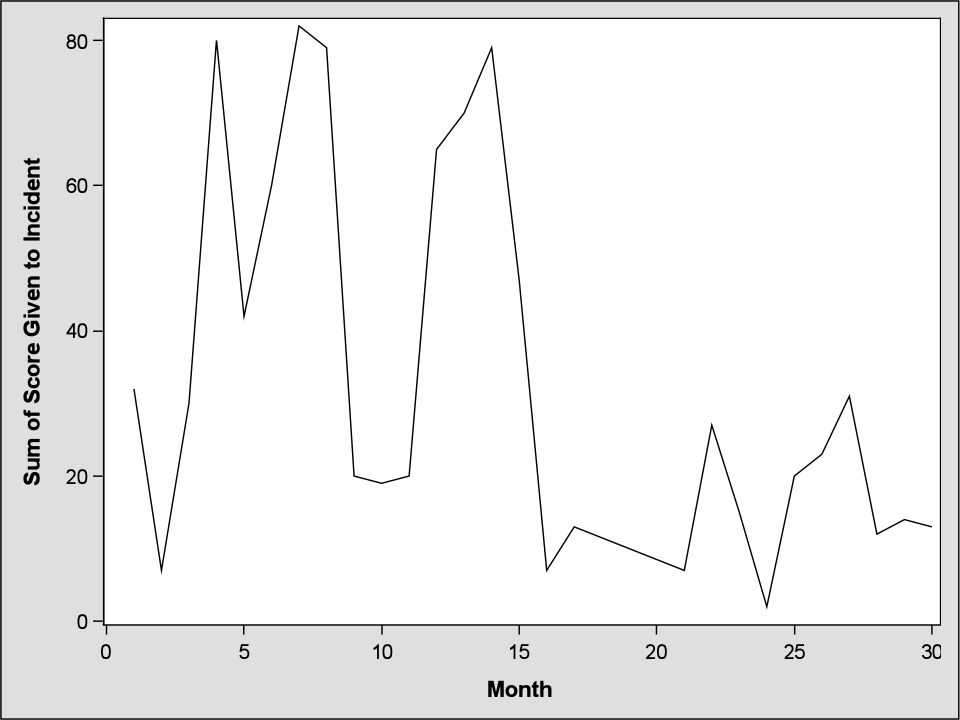
\includegraphics[scale=0.25]{Pic/Q1/1.png}
	\caption{Sequence Diagram}
	\label{f1}
\end{figure}

Based on figure of \ref{f1}, the sequence has no significant non-stationary features. White noise detection shows that there is a correlation between the sequence values, which is a non white noise sequence.

Secondly, I use three methods to solve the best parameters, namely MINIC, SCAN, and ESACF. The results of them are shown in table \ref{t1}.

\begin{table}[H]
	\centering

\begin{longtable}{rrrrrr}
\toprule
	\multicolumn{3}{c}{SCAN} &    \multicolumn{3}{c}{ESACF}\\
	\midrule
    p+d &    q &    BIC &    p+d &    q &    BIC\\
\endhead
    1 &    0 &    5.405064 &    1 &    0 &    5.405064\\
    0 &    1 &    5.60567 &    0 &    1 &    5.60567\\
     &      &      &    4 &    0 &    5.152248\\
     &      &      &    5 &    0 &    5.066185\\
\bottomrule

\caption{ARMA(p+d,q) Tentative Order Selection Tests}
\label{t1}
\end{longtable}
\end{table}

The results show that MA(5) model should be chosen. The ARIMA module of SAS is used to implement the model. After adjusting the parameters to P = 0 and Q = 5, the model results are shown in the following figure \ref{t2}.

\begin{table}[H]
\centering
\begin{longtable}{lrrrrr}
\toprule
   Parameter &    Estimate &    Standard {\newline} Error &    t~Value &    Approx {\newline} Pr > |t| &    Lag\\
\endhead
\midrule
   MU &    35.06369 &    8.46743 &    4.14 &    0.0005 &    0\\
   MA1,1 &    $-$0.69146 &    0.21930 &    $-$3.15 &    0.0048 &    1\\
   MA1,2 &    $-$0.28225 &    0.26805 &    $-$1.05 &    0.3043 &    2\\
   MA1,3 &    0.04334 &    0.28187 &    0.15 &    0.8793 &    3\\
   MA1,4 &    $-$0.02787 &    0.27443 &    $-$0.10 &    0.9201 &    4\\
   MA1,5 &    0.01157 &    0.22909 &    0.05 &    0.9602 &    5\\
\bottomrule
\caption{Conditional Least Squares Estimation of MA(5)}
\label{t2}
\end{longtable}

\begin{longtable}{lr}
\toprule
   Constant Estimate &    35.06369\\
   Variance Estimate &    552.6743\\
   Std Error Estimate &    23.50903\\
   AIC &    252.3359\\
   SBC &    260.111\\
   Number of Residuals &    27\\
\bottomrule
\caption{Model Diagnosis of MA(5)}
\label{t3}
\end{longtable}
\end{table}

According to the table \ref{t2}, we found that only two coefficients are significant. Therefore, the model should be redraft. After I calculated 121 models with P from 0 to 10 as well as Q between 0 and 10, AR(1) need to be considered since the AIC is the lowest in these models. The result of the models was given as follow.

\begin{table}[H]
\centering
\begin{longtable}{lrrrrr}
\toprule
   Parameter &    Estimate &    Standard {\newline} Error &    t~Value &    Approx {\newline} Pr > |t| &    Lag\\
\endhead
\midrule
   MU &    32.87074 &    9.17622 &    3.58 &    0.0014 &    0\\
   AR1,1 &    0.56566 &    0.16798 &    3.37 &    0.0025 &    1\\
\bottomrule
\caption{Conditional Least Squares Estimation of AR(1)}
\label{t4}
\end{longtable}
\end{table}

\begin{table}[H]
\centering
\begin{longtable}{lr}
\toprule
   Constant Estimate &    14.27693\\
   Variance Estimate &    495.1036\\
   Std Error Estimate &    22.25092\\
   AIC &    246.0734\\
   SBC &    248.6651\\
   Number of Residuals &    27\\
\bottomrule
\caption{Model Diagnosis of AR(1)}
\label{t5}
\end{longtable}
\end{table}

Comparing table \ref{t3} and \ref{t5}, we obtain the conclusion that AR(1) is much more appropriate than MA(5). In addition,, the parameters of AR(1) are significant since p-values are both less than 0.05 (Figure \ref{f2}).


\begin{figure}[H]
\centering
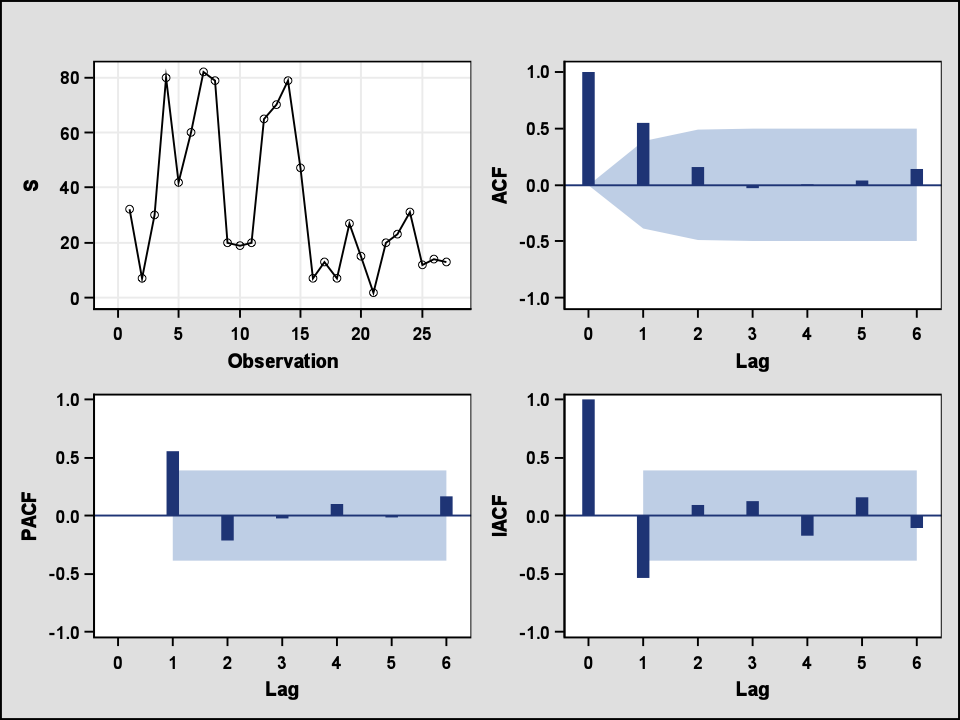
\includegraphics[scale=0.25]{Pic/Q1/2.png}
\caption{Trend and Correlation Analysis for Sum of Score Given to Incident}
\label{f2}
\end{figure}

Thirdly, according to the autocorrelation coefficient in figure \ref{f2}, except for the autocorrelation coefficients of the first order delay being instead of are in the range of twice standard deviation, the autocorrelation coefficients of other orders fluctuate in the range of twice standard deviation. Based on this feature, we can judge that the sequence has short-term correlation, and further confirm that the sequence is stable. Furthermore, the process of the partial autocorrelation coefficient decaying to zero is further investigated. Except the first order partial autocorrelation coefficient being instead of is in the range of double standard deviation, the other order partial autocorrelation coefficients are in the range of double standard deviation, which is a typical characteristic of the first-order truncated partial autocorrelation coefficient.

Finally, according to the table \ref{t4}, the fomula of AR(1) can be demonstrated as follow.

\begin{equation}
x_{t} = 32.87074 + 0.56566\times x_{t-1} + \epsilon_{t}, Var(\epsilon_{t}) = 495.1036
\label{e1}
\end{equation}

where $x_{t}$ is sum of score given to incident by month t.

\begin{figure}[H]
\centering
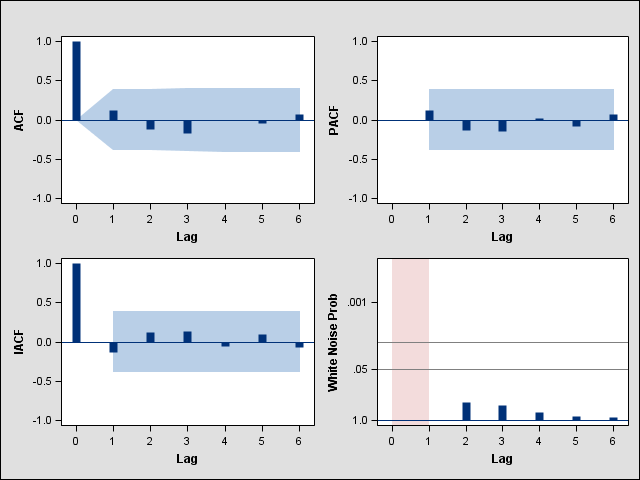
\includegraphics[scale=0.5]{Pic/Q1/3.png}
\caption{Residual Correlation Diagnostics for Sum of Score Given to Incident}
\label{f3}
\end{figure}

\begin{figure}[H]
\centering
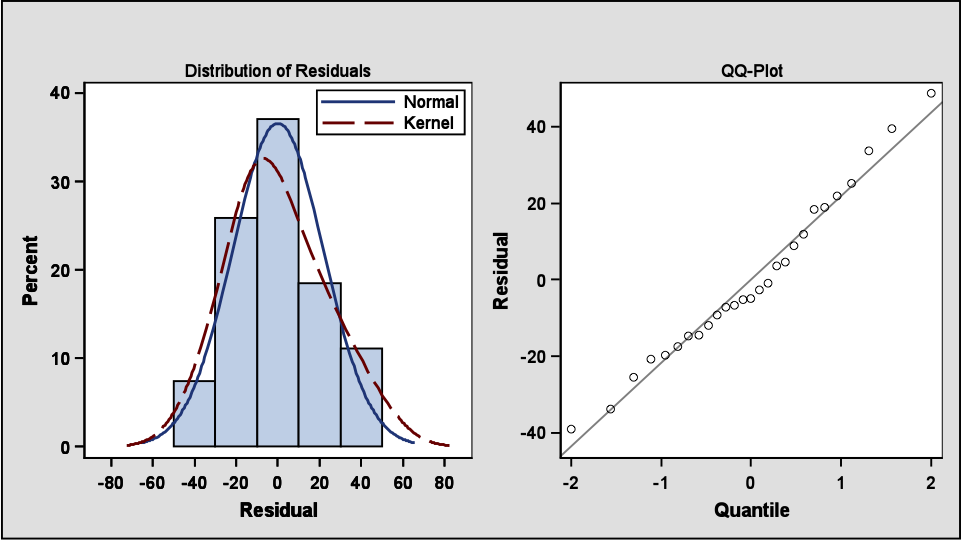
\includegraphics[scale=0.25]{Pic/Q1/4.png}
\caption{Residual Normality Diagnostics for Sum of Score Given to Incident}
\label{f4}
\end{figure}

These two figures (\ref{f2}, \ref{f3}) show that the effect of the model is good. The residual error of the model is in line with normal distribution from the chart of QQ plot.

\subsection*{Hypothesis testing}

The significance test of model \ref{e1} is white noise test of residual sequence. Therefore, the null hypothesis and alternative hypothesis are:

$$H_{0}: \rho_{1} = 0, \forall m \ge 1$$
$$H_{1}: \exists \rho_{k}\neq 0, \forall m \ge 1, k\le m$$

The test statistic is LB (Ljung-Box):

$$LB = n(n + 2) \sum_{k=1}^{m}(\frac{\hat{\rho_{k}}^{2}}{n-k})\sim \chi^{2}(m), \forall m > 0$$

If the null hypothesis is rejected, it means that there are still some relevant information in the residual sequence, and the fitting model is not significant. If the original hypothesis cannot be rejected, the fitting model is considered significant. The result is given as table \ref{tlb}.

\begin{table}[H]
\begin{longtable}{rrrrrrrrrr}
\toprule
   To Lag &    Chi-Square &    DF &    Pr > ChiSq &    \multicolumn{6}{c}{Autocorrelations}\\
  \midrule
\endhead
   6 &    10.73 &    6 &    0.0969 &    0.551 &    0.155 &    $-$0.032 &    0.002 &    0.036 &    0.142\\
\bottomrule
\caption{Autocorrelation Check for White Noise}
\label{tlb}
\end{longtable}
\end{table}

It can be seen from the results that p-value is 0.0969, which is greater than 0.05. Therefore, we cannot reject the null hypothesis. This is a good proof that the data is a very stable white noise sequence. In conclusion, this model proves the fact that the trends in violence is non-monotonic over time. The option D may be the correct answer.
